\section{Maximal Closure}

We can start this section with an example:\\
\begin{figure}[!h]
\centering
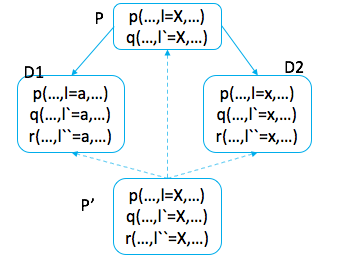
\includegraphics[width=250pt]{./pictures/0305.png}
\caption{Specific Pattern may exist}
\end{figure}
From the example we can see that, $D_1\preceq P$ is realized by $\theta_1= \{X=a\}$, and $D_2\preceq P$, by $X=x, Y=y$.\\
we can find a more specific $P' = {p(X,X),q(X)}$, makes that $D_1\preceq P$ but not $D_2\preceq P'$.\\
In a more simple situation, we may have two documents $D_1$ and $D_2$ , and a pattern $P$.
\begin{displaymath}
D_1 = \{p(l_1 = a, l_2 = a),q(l_1 = a)\}
\end{displaymath}
\begin{displaymath}
D_2 = \{p(l_1 = x, l_2 = y),q(l_1 = x)\}
\end{displaymath}
\begin{displaymath}
P = \{p(l_1 = X, l_2 = Y),q(l_1 = X)\}
\end{displaymath}
Thus, $a\in D_1$ and $x\in D_2$ plays the same role $ A_1 = {p(l_1),q(l_1)}$ represented by variable $X$.\\
As another shared role, $A_2 = {p(l_2)}$ , played by $a\in D_1$ and $y\in D_2$ and corresponding to $Y$.
Similarity class is a set of constants that play the same role $R \subseteq \mathcal{R}$ defined by the descriptive pattern. Durning the search process for the descriptive pattern, the exact similarity classes are also under investigation. We use the following sufficient condition for the similarity defined by the descriptive pattern.
\begin{enumerate}
\item for patterns $P_1\prec P_2$ realized by variable substitution $\theta$,
\begin{displaymath}
role_{P_2} (X) \subset role_{P_1} (X\theta)\ for\ X \in Var(P_2)
\end{displaymath}
That means role set represented by variable increases by specialization.
\item for a role set $\mathcal{R}$ ,we have
\begin{displaymath}
|[R]| = \{D\in \mathcal{D}|\psi_DR\ne \emptyset\}
\end{displaymath}
and,
\begin{displaymath}
|[R]| = \{D\in \mathcal{D}|\psi_DR\ne \emptyset\ and \ \max_{a\in const(D)}keyscore_D(a)\leq \kappa\}
\end{displaymath}
\item for a descriptive pattern $P$ and variable $X \in Var(P)$ , $R = role_P (X)$ is a maximal role set among role set $R'$, generated by a pattern. 
\end{enumerate}
Support $\mathcal{R}$ is a role set from descriptive pattern $P$ , if we can find a more specific $P'$ , it will lead inconsistency if the role set is not maximal. To make sure pattern $P$ is minimal among all satisfying ones, we have to maximize role set.\\
\begin{figure}[!h]
\centering
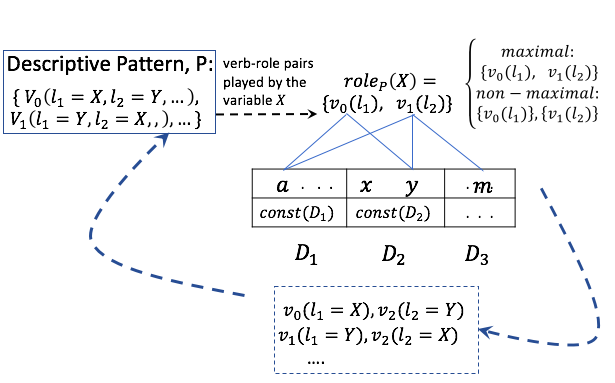
\includegraphics[width=300pt]{./pictures/0305-0.png}
\caption{Maximal closure is a complete set}
\end{figure}
We can use both Formal Concept Analysis or CLIQUE idea to extract maximal role set from our data. In my research, we use bipartite clique idea to solve the problem, because it is a more simple idea to understand the input and output, without learning more specific knowledge. We can understand the idea of bipartite clique to extract maximal closure of role set in the figure below,\\
\begin{figure}[!h]
\centering
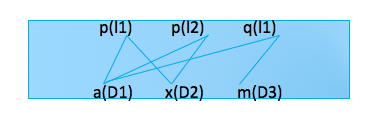
\includegraphics[width=250pt]{./pictures/0305-1.png}
\caption{there exists maximal bipartite clique with role set smaller than others}
\end{figure}
\begin{fact}
Actually, Maximal clique and Formal Concept have the same meaning. consider bipartite graph $(const(D),R,E)$ , where incident rel $E\subseteq const(D) \times R$ is defined by
\begin{displaymath}
C \iff FC<C \cap const(D),C\cap R>
\end{displaymath}
\end{fact}
\begin{proof}Sufficiency and Necessary,\\
Sufficiency: We cannot add new $D$ or $R$ elements to $C$. Hence, letting $A = C\cap R$,
\begin{displaymath}
\psi A = C\cap const(D)\ and\ A = \varphi\psi A
\end{displaymath}
Necessary: for $A = C \cap R$ and $\psi A = C \cap const(D)$ , as $A$ is a closure, we cannot add new role. as $\psi A$ is also an object closure, we cannot add new const.
\end{proof}
The processing of maximizing role set is as follow,\\
initial candidate set ${p(l)||[p(l)]| >\kappa}$,
\begin{displaymath}
Cand(R) = \{a\ role\ p(l)\notin R||D\in\mathcal{D}|\psi(R\cup\{p(l)\})\cap const(D)\ne \emptyset \}\ne N_\tau \}
\end{displaymath}
Of course, the candidate should meet the condition of KeyGraph,
\begin{displaymath}
maxKeyscore(\psi(R\cup\{p(l)\})\cap const(D))\geq\kappa
\end{displaymath}